\documentclass{article}
\usepackage[utf8]{inputenc}
\usepackage{amsmath, amssymb, amsthm}
\usepackage{graphicx, float}
\usepackage{hyperref}
\usepackage[dvipsnames]{xcolor}
\usepackage{algorithm}
\usepackage[noend]{algpseudocode}
\graphicspath{{../Images/}}

% Customization of the document
\usepackage[letterpaper, top=1.8cm, bottom=2.3cm, left=2cm, right=2cm, heightrounded]{geometry}

% Line height
\renewcommand{\baselinestretch}{1.15}

% Define the exercise counter
\newcounter{exercise}[section]   % Resets the counter every time you change the section

% Format of exercise number (e.g., 1.1-1, 1.1-2, ...)
\renewcommand{\theexercise}{\thesection.\arabic{exercise}}

% Parskip and parindent
\setlength{\parindent}{0pt}
\setlength{\parskip}{0.8em}

\title{Exercise of Getting Started}
\author{Grabur}
\date{Feb 2025}

\begin{document}

\maketitle

\section{Chapter 1: Foundations}

\subsection{The Role of Algorithms in Computing}
I didn't make the exercise of this section because I didn't find them useful.

\subsection{Getting Started}
\setcounter{exercise}{0} % Start from 0 for the exercises in this section

% Used to make a label for referencing later if it's necesary
\refstepcounter{exercise}
\textbf{Exercise 1.2-1)}:\\
It could be an application like booking. When you search a hotel close to the airport, 
it gets involved algorithms as searching the hotels close to that airport and it should be
searched in a short time period.

\refstepcounter{exercise}
\textbf{Exercise 1.2-2)}:\\
\begin{flalign*}
    8n^2 < 64n \cdot \log_2 n \quad \rightarrow \quad n < 8 \cdot \log_2 n
\end{flalign*}
Try values until this inequality is false. To $n \lessapprox 43$, insertion sort runs 
faster than merge sort.

\refstepcounter{exercise}
\textbf{Exercise 1.2-3)}:\\
\begin{flalign*}
    100n^2 < 2^n \quad 
\end{flalign*}
Trying values, for $n \lessapprox 15$, $2^n$ runs faster than $100n^2$.

\refstepcounter{exercise}
\textbf{Exercise 1.2-4)}:\\
\\
\textit{\large View photo of the exercise on the next page.}
\newpage
\begin{figure*}[h]
    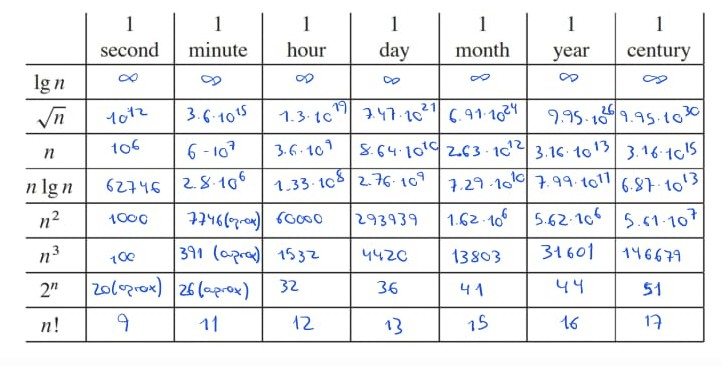
\includegraphics[scale=0.5]{Problem1_1}
    \centering
\end{figure*}


\refstepcounter{exercise}
\textbf{Exercise 2.1-1)}:\\
Note: Resolved using the logic of C, C++, Java, etc. while iterating over an array on a for
loop. Also the number that appears in \textcolor{ForestGreen}{green}, is the number being 
checked. The number or numbers that appears in \textcolor{Red}{red} are the numbers being 
moved.

\begin{center}
    \begin{tabular}{|c|c|}
    \hline
    \textbf{i} & \textbf{Array} \\
    \hline
    1) & [31, \textcolor{ForestGreen}{41}, 59, 26, 41, 58]\\
    2) & [31, 41, \textcolor{ForestGreen}{59}, 26, 41, 58]\\
    3) & [\textcolor{ForestGreen}{26}, \textcolor{Red}{31}, \textcolor{Red}{41}, 
          \textcolor{Red}{59}, 41, 58]\\
    4) & [26, 31, 41, \textcolor{ForestGreen}{41}, \textcolor{Red}{59}, 58]\\
    5) & [26, 31, 41, 41, \textcolor{ForestGreen}{58}, \textcolor{Red}{59}]\\
    \hline
    \end{tabular}
\end{center}

\refstepcounter{exercise}
\textbf{Exercise 2.1-2)}:\\
\textbf{Initialization}: The loop start getting the first number in the array. In spite of 
that, it has initialized to 0 the variable sum where the total sum will be stored. Due to 
that, the invariant holds the first number that will be added to sum.

\textbf{Maintenance}: On each iteration, the loop will hold only the index of the number 
that will be added, after add it, i will be incremented by 1, holding the next number (i + 1).

\textbf{Termination}: The loop will terminate when the 'n' elements of the array are added. In conclusion,
sum it's equivalent of say that $sum = \sum_{i = 1}^{n} A[i]$.
    
\refstepcounter{exercise}
\textbf{Exercise 2.1-3)}:\\
click this link to see the resolution \(\rightarrow \href{https://github.com/Graburr/Algorithms_CLRS_4ed_solutions/blob/main/chapter1/Getting_Started/2.1-3.cpp}
{\textcolor{blue}{resolution}}\)

\refstepcounter{exercise}
\textbf{Exercise 2.1-4)}:\\
\begin{algorithm}
\caption{Linear Search}\label{linearSearchID}
\begin{algorithmic}[1]
\Function{Linear-Search}{$A, n, x$}
    \For{$i \gets 1$ \textbf{to} $n$}
        \If {$ A[i] == x $} 
            \Return $i$
        \EndIf
    \EndFor
    \State \Return \textit{NIL}
\EndFunction
\end{algorithmic}
\end{algorithm}

\textbf{Initialization}: The loop start getting the first element of the array. 

\textbf{Maintenance}: On each iteration, the loop takes the next element (i + 1) and compare 
it with the value being search (x). If it's found return i, else, continue searching that 
value.

\textbf{Termination}: When all values are read, if x wasn't found in the array, it returns
NIL to indicate that no value was found on all the array.

\refstepcounter{exercise}
\textbf{Exercise 2.1-5)}:\\
\begin{algorithm}
\caption{ADD-BINARY-INTEGERS}\label{AddBinarySearchID}
\begin{algorithmic}[1]
\Function{ADD-BINARY-INTEGERS}{$A, B, n$}
    \State \textit{//Initialize array C with n values}
    \State \textit{carry} $\gets 0$ 
    \For {$i \gets 1$ \textbf{to} $n$}
        \State $c \gets A[i] + B[i]$
        \State $C[i] \gets c \mod 2$
        \State $carry \gets c \div 2$ \quad \textit{//Integer division}
    \EndFor
    \Statex
    \State $C[n] \gets carry$
    \State \Return \textit{C} \quad \textit{//Return the array C with the values}
\EndFunction
\end{algorithmic}
\end{algorithm}

\textbf{Initialization}: The loop starts with value of carry to 0, and getting the first 
bits of A and B.

\textbf{Maintenance}: On each iteration, the loop takes the next bits values of A and B.
Add these values and calculate the value to insert into C and the carry that could exists.

\textbf{Termination}: All values were added and store, now C[0:n - 1] with the result of 
the sum. To reach the n-th value, adds the last carry value on the position n.

\refstepcounter{exercise}
\textbf{Exercise 2.2-1)}:\\
Like the book says, \(\Theta\) notation is like saying "roughly proportional to \(n^2\) (for example), 
when \(n\) is large." In this case, we remove constants, so the remaining expression is 
\(n^3 + n^2 + n + 3\). The term with the highest exponent is \(n^3\), so at any moment:
\(n^3 \gg n^2 \gg n\). \\ 
\textbf{Solution}: \(\Theta(n^3)\).

\refstepcounter{exercise}
\textbf{Exercise 2.2-2)}:\\
\begin{algorithm}
\caption{SELECTION-SORT}\label{SelectionSortID}
\begin{algorithmic}[1]
\Function{SELECTION-SORT}{$A, n$}
    \For{$i \gets 1$ \textbf{to} $n - 1$}
        \State $ind\_small\_elm \gets i$
        \For{$j \gets i + 1$ \textbf{to} $n$}
            \If{$A[ind\_small\_elm] > A[j]$}
                \State $ind\_small\_elm \gets j$
            \EndIf
        \EndFor
        \State \Call{swap}{$A[i], A[ind\_small\_elm]$}
    \EndFor
\EndFunction
\end{algorithmic}
\end{algorithm}

The invairant is that on each iteration of extern for, it only takes 1 by 1 element. In the
inner for, also take all elemnts from i to n, and compare the value of the outter for
against the inner for to take the smaller elemnt.

When the algorithm arrives to the last element, all swaps ocurred and the last element will
be in the correct place.

The worst case happens when it must iterate on the outher for and also with al the elements
from i to n in the inner for. So it's: \(\frac{n*(n - 1)}{2}\). Thats mean that avoiding all
constants values, the solution is: \(\Theta(n^2)\).

The best case is not better because you have to check all values in the if, the only instruction
that is avoided is the instruction inside the if because the if won't be evaluated to true.
But that instruction is insignificant if \(n\) it's too big.

\refstepcounter{exercise}
\textbf{Exercise 2.2-3)}:\\
Depends on the value where is storage, if the \(x\) value is storage at the first position it
will take a constant value to search it. However, if the value is in the last element 
(worst case) it will spend \(constant * n\) time to find that value.

Averege case is suposing that it's in the middle of the array. The averegage is \(\frac{n}{2} = n\)
if \(n\) it's too big. 

Worst case as mentioned before is \(\Theta(n)\).

\refstepcounter{exercise}
\textbf{Exercise 2.2-3)}:\\
The only thing you could do is a preprocessing step to check if it's alredy sorted or nearly
to be sorted and then apply the algorithm who best fits when the best case was achieved.



\end{document}
